%%%%%%%%%%%%%%%%%%%%%%%%%%%%%%%%%%%%%%%%%%%%%%%%%%%%%%%%%%%%%%%%%%%%
%% I, the copyright holder of this work, release this work into the
%% public domain. This applies worldwide. In some countries this may
%% not be legally possible; if so: I grant anyone the right to use
%% this work for any purpose, without any conditions, unless such
%% conditions are required by law.
%%%%%%%%%%%%%%%%%%%%%%%%%%%%%%%%%%%%%%%%%%%%%%%%%%%%%%%%%%%%%%%%%%%%

\documentclass[
  digital,     %% The `digital` option enables the default options for the
               %% digital version of a document. Replace with `printed`
               %% to enable the default options for the printed version
               %% of a document.
%%  color,       %% Uncomment these lines (by removing the %% at the
%%               %% beginning) to use color in the printed version of your
%%               %% document
  oneside,     %% The `oneside` option enables one-sided typesetting,
               %% which is preferred if you are only going to submit a
               %% digital version of your thesis. Replace with `twoside`
               %% for double-sided typesetting if you are planning to
               %% also print your thesis. For double-sided typesetting,
               %% use at least 120 g/m² paper to prevent show-through.
  nosansbold,  %% The `nosansbold` option prevents the use of the
               %% sans-serif type face for bold text. Replace with
               %% `sansbold` to use sans-serif type face for bold text.
  nocolorbold, %% The `nocolorbold` option disables the usage of the
               %% blue color for bold text, instead using black. Replace
               %% with `colorbold` to use blue for bold text.
  lof,         %% The `lof` option prints the List of Figures. Replace
               %% with `nolof` to hide the List of Figures.
  lot,         %% The `lot` option prints the List of Tables. Replace
               %% with `nolot` to hide the List of Tables.
]{fithesis4}
%% The following section sets up the locales used in the thesis.
\usepackage[resetfonts]{cmap} %% We need to load the T2A font encoding
\usepackage[
  main=english, %% By using `czech` or `slovak` as the main locale
                %% instead of `english`, you can typeset the thesis
                %% in either Czech or Slovak, respectively.
  % english, german, russian, czech, slovak %% The additional keys allow
]{babel}        %% foreign texts to be typeset as follows:
%%
%%   \begin{otherlanguage}{german}  ... \end{otherlanguage}
%%   \begin{otherlanguage}{russian} ... \end{otherlanguage}
%%   \begin{otherlanguage}{czech}   ... \end{otherlanguage}
%%   \begin{otherlanguage}{slovak}  ... \end{otherlanguage}
%%
%% For non-Latin scripts, it may be necessary to load additional
%% fonts:
\usepackage{paratype}
% \def\textrussian#1{{\usefont{T2A}{PTSerif-TLF}{m}{rm}#1}}
%%
%% The following section sets up the metadata of the thesis.
\thesissetup{
    date        = \the\year/\the\month/\the\day,
    university  = mu,
    faculty     = fi,
    type        = bc,
    department  = Department of Computer Systems and Communications,
    author      = Dominik Tichý,
    gender      = m,
    advisor     = {RNDr. Tomáš Raček, Ph.D.},
    title       = {Modern visualization of partial atomic charges in Mol*},
    TeXtitle    = {Modern visualization of partial atomic charges in Mol*},
    keywords    = { Molstar, molecular visualization, partial atomic charges },
    TeXkeywords = { TODO },
    abstract    = {%
        TODO
    },
    thanks      = {%
        TODO
    },
    % bib         = example.bib,
    %% Remove the following line to use the JVS 2018 faculty logo.
    facultyLogo = fithesis-fi,
}
\usepackage{makeidx}      %% The `makeidx` package contains
\makeindex                %% helper commands for index typesetting.
%% These additional packages are used within the document:
\usepackage{paralist} %% Compact list environments
\usepackage{amsmath}  %% Mathematics
\usepackage{amsthm}
\usepackage{amsfonts}
\usepackage{url}      %% Hyperlinks
\usepackage{markdown} %% Lightweight markup
\usepackage{listings} %% Source code highlighting
\lstset{
  basicstyle      = \ttfamily,
  identifierstyle = \color{black},
  keywordstyle    = \color{blue},
  keywordstyle    = {[2]\color{cyan}},
  keywordstyle    = {[3]\color{olive}},
  stringstyle     = \color{teal},
  commentstyle    = \itshape\color{magenta},
  breaklines      = true,
}
\usepackage{floatrow} %% Putting captions above tables
\floatsetup[table]{capposition=top}
\usepackage[babel]{csquotes} %% Context-sensitive quotation marks

\begin{document}

\chapter*{Introduction}
\markright{\textsc{Introduction}}
\addcontentsline{toc}{chapter}{Introduction}

\chapter{Theory}
\label{chapter:theory}

Theoretical concepts are fundamental to the study of computational chemistry, providing a framework for analyzing molecular structures and properties. This chapter focuses on four key areas of theory, beginning with an overview of molecular structure in Section 1.1. Section 1.2 provides an in-depth examination of chemical file formats, including the advantages and disadvantages of different file formats for storing molecular data. Partial atomic charges are explored in section 1.3, including their importance in the analysis of molecular structures and the various methods used to compute them. Finally, section 1.4 delves into color interpolation, a critical technique for visualizing partial atomic charges in molecular structures.

By providing a comprehensive overview of these theoretical concepts, this chapter aims to provide a strong foundation for the subsequent chapters, which will focus on the implementation and analysis of the Molstar extension for visualizing partial atomic charges in molecular structures.

\section{Molecular structure}
\label{section:molecular_structure}

Molecular structure refers to the arrangement of atoms and chemical bonds in a molecule. The three main components of molecular structure are atoms, residues, and chains.
In this section we will look at

\subsection{Atoms}
\label{subsection:atoms}

Atoms are the basic building blocks of matter. Atoms are composed of protons, neutrons, and electrons. The number of protons determines the element, while the number of neutrons determines the isotope. The number of electrons determines the charge of the atom. Atoms are the smallest unit of matter that can take part in a chemical reaction.

Bonds are the connections between atoms that hold molecules together. There are different types of bonds, e.g. covalent bonds, ionic bonds, and hydrogen bonds.

\subsection{Residues}
\label{subsection:residues}

A residue refers to a specific building block that remains after a chemical modification or enzymatic reaction.
In proteins, residues refer to amino acids, which are connected through peptide bonds to form polypeptide chains.
Residues are crucial in biochemistry because they determine the structure and function of biological molecules.
The sequence of residues in a protein or nucleic acid, for instance, determines its three-dimensional structure and ultimately its biological activity.

\subsection{Chains}
\label{subsection:chains}

Polymer chains (chains) are sequences of residues that are linked together. In the context of biomolecules, chains can be either polypeptide chains in proteins or polynucleotide chains in nucleic acids. The sequence and structure of these chains are crucial for understanding the function and properties of the biomolecules.

\section{Chemical file formats}
\label{section:chemical_file_formats}

TODO: introduction

\subsection{SDF}
\label{subsection:sdf}

Structure-data file (SDF) is a widely used chemical file format for representing molecular structures and their associated properties. It is a text-based format that describes the atoms, bonds, and atomic coordinates of a molecule. 

\subsection{MOL2}
\label{subsection:mol2}

The Mol2 file format is another text-based format for storing molecular structures and their associated properties. It can store multiple conformations of a molecule and is commonly used in molecular modeling and cheminformatics applications. The Mol2 format provides more flexibility and additional features compared to the SDF format, such as support for multiple substructures and atom types.

\subsection{PDB}
\label{subsection:pdb}

The Protein Data Bank (PDB) file format is a widely used format for storing three-dimensional structures of proteins, nucleic acids, and other macromolecules. PDB files contain information about the atomic coordinates, secondary structure, and other important details required for understanding macromolecular structures. The PDB format has been widely adopted in structural biology, bioinformatics, and related fields.

\subsection{mmCIF}
\label{subsection:mmcif}

The macromolecular Crystallographic Information File (mmCIF) format is an extension of the CIF format, specifically designed for macromolecular structures.
It is a text-based format that provides a more comprehensive and flexible representation of macromolecular crystallography data compared to the PDB format.
One of the most important features of the mmCIF format is its support for data dictionaries.
This allows users to define new data items and integrate additional information.
In contrast to other formats, the mmCIF format does not impose limits on column width and entry count, making it more flexible and accommodating for storing large amounts of data.

TODO: add example image + better explanation

\section{Partial atomic charges}
\label{section:partial_atomic_charges}

Partial atomic charges are a measure of the distribution of electronic charge within a molecule. These charges are important for understanding and predicting molecular interactions, including hydrogen bonding, electrostatic interactions, and solvation effects.

TODO: visual of electron distribution

\subsection{Calculation methods}
\label{subsection:calculation_methods}

\subsection{ChargeFW2}
\label{subsection:chargfw2}

\subsection{AlphaCharges}
\label{subsection:alphacharges}

\section{Color interpolation}
\label{section:color_interpolation}

Color interpolation is the process of creating new colors by mixing two or more colors together. It is a common technique used in computer graphics and digital image processing to create smooth transitions between colors.

Color interpolation works by calculating the intermediate colors between two or more given colors. This is typically done by taking a weighted average of the red, green, and blue values of the colors being interpolated.

TODO: add math equation + image of red,white and white,blue interpolation

\chapter{Visualizing molecular data}
\label{chapter:visualizing_molecular_data}

This chapter will discuss various types of visualizations, the role of coloring in molecular representations, and some commonly used software tools for creating these visualizations.

\section{Types of visualizations}
\label{section:types_of_visualizations}

There are several methods to represent molecular data, each with its own benefits and drawbacks. The methods most relevant to this work are the following three types: ball and stick, surface, and cartoon.

\subsection{Ball and stick}
\label{subsection:ball_and_stick}

The ball and stick model represents atoms as spheres and bonds as cylindrical connections between these spheres. This model provides a simple and intuitive visualization of a molecule's atomic structure. It highlights individual atoms and their bonds, including their bond types. However, it may not accurately represent the spatial relationships between atoms in larger molecules or macromolecular complexes.

\subsection{Surface}
\label{subsection:surface}

Surface representations depict the three-dimensional shape of a molecule by displaying its solvent-accessible surface.
This model provides a more accurate representation of the molecule's overall shape and size, making it especially useful for studying macromolecular interactions and the binding of small molecules.
For example, surface visualization can be used to identify potential binding sites on a protein surface, which can then be targeted by drug molecules.

\subsection{Cartoon}
\label{subsection:cartoon}

Cartoon representations simplify the molecular structure by focusing on the secondary structure elements of proteins and nucleic acids, such as alpha helices, beta sheets, and loops. Alpha helices are often depicted as a spiral-like structures, whereas beta sheets as arrows. This type of visualization is particularly useful for visualizing large macromolecular complexes, as it highlights the overall organization and topology of the molecule without the clutter of atomic details. The simplification of the structure also makes it easier to understand the folding and dynamics of the molecule.

\subsection{Coloring of molecular visualizations}
\label{subsection:coloring_of_molecular_visualizations}

Coloring is an essential aspect of molecular visualization, as it can provide additional information and help to emphasize specific features or properties of the molecule. Some common coloring schemes include:
- By element: Atoms are colored according to their chemical element (e.g., carbon in grey, oxygen in red, nitrogen in blue).
- By partial atomic charge: Atoms or residues are colored according to their charge or charge sum. Negative charges are depicted in red, positive charges in blue.

\section{Visualization software}
\label{section:visualization_software}

There are numerous software tools available for visualizing molecular data, with varying levels of complexity, customization, and features. Two widely used tools are LiteMol and Mol*.

\subsection{Litemol}
\label{subsection:litemol}

LiteMol is an open-source, web-native molecular visualization tool that supports various file formats and offers a user-friendly interface for creating visualizations. LiteMol provides essential visualization types, including ball and stick, surface, and cartoon representations, as well as options for customizing colors, lighting, and other display settings. The web-based nature of LiteMol makes it easily accessible and platform-independent.

\subsection{Molstar}
\label{subsection:molstar}

Mol* (Molstar) is another web-native molecular visualization tool, developed as part of the wwPDB OneDep system for macromolecular structure deposition and validation. Mol* offers a wide range of visualization options, including advanced features such as electron density maps and validation reports. Mol* supports many file formats, including PDB, mmCIF, and PDBx/mmJSON. Like LiteMol, Mol* is platform-independent and can be accessed from any web browser.

Mol* emphasizes interactivity and offers various tools for manipulating and analyzing the molecular structure, such as distance and angle measurements, selection and display of specific residues, and custom coloring schemes. Additionally, Mol* provides integration with external databases and services, such as UniProt, PDBe, and RCSB PDB, enabling users to quickly access related information and resources.

\chapter{Molstar partial charges extension}
\label{chapter:molstar_partial_charges_extension}

Visualizing partial atomic charges in molecules is an essential aspect of computational chemistry research, aiding in analyzing complex molecular structures. Molstar, a popular software tool for visualizing molecules, provides an extensive range of features for users to explore molecular structures. However, the tool lacks the functionality to color and label atoms and residues based on their partial atomic charges. This can be a significant limitation for researchers. In response to this need, we have created an extension to Molstar that addresses this limitation.

This chapter describes the requirements for the extension, the custom mmCIF categories necessary for storing the partial atomic charges, and the implementation of the extension itself.

\section{Requirements}
\label{section:requirements}

This section briefly describes the formal requirements for the Molstar extension. Firstly, the extension should enable the coloring of atoms and residues based on their partial atomic charges. Secondly, it should describe the charge values of the atoms and residues. Lastly, the extension should be seamlessly integrated into the Molstar library, facilitating access to its features regardless of the Molstar viewer instance.
TODO: the extension should also support multiple charges sets

\section{Custom mmCIF categories}
\label{section:custom_mmcif_categories}

However, in order to store partial atomic charges within a single file, we needed to create custom categories within the mmCIF format.
The design of these custom categories was a crucial step in creating the extension since we needed a way to package the charge data together with the structure data into one file.

Without having everything in one file we would have to provide the charges in a different way e.g. through custom import controls.

For this purpose we have chosen the mmCIF file format. There are a couple of reasons already discussed in section 1.2 as to why mmCIF is more advance file format than the other formats discussed in section 1.2. For our purposes the biggest advantage was the ease of creating custom data categories for describing data relating to the partial atomic charges.

The custom categories allowed us to store information about the partial atomic charges separately from the other structural data.

We used two separate categories for storing the charge data.
The first category stores the partial charge values for each atom in the structure. The binding of atom and its charge is done using an attribute atom\_id which is a pointer to the atom\_site.id. item. Additionally, we use an attribute typeId as a pointer into the second category which is dedicated to storing metadata about the charge sets.

The metadata category has three attributes - id, type, and method. Attribute id is a unique identifier for the charge set, attribute type serves to describe the type of computation method used (e.g. empirical, quantum etc.), and lastly the method attribute describes the method name with parameters if applicable (e.g. 'EEM/Racek 2016 (ccd2016\_npa)').

Figure \ref{fig:mmcif_erd} provides a detailed illustration of the structure of the custom mmCIF categories.

\begin{figure}
  \begin{center}
    %% PNG and JPG images can be inserted into the document as well,
    %% but their resolution needs to be adequate. The minimum is
    %% about 100 pixels per 1 centimeter or 300 pixels per 1 inch.
    %% That means that a JPG or PNG image typeset at 4 × 4 cm should
    %% be 400 × 400 px large at the bare minimum.
    %%
    %% The optimum is about 250 pixels per 1 centimeter or 600
    %% pixels per 1 inch. That means that a JPG or PNG image typeset
    %% at 4 × 4 cm should be 1000 × 1000 px large or larger.
    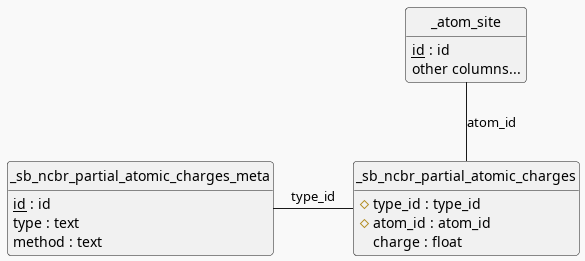
\includegraphics[width=10cm]{figures/mmcif_erd.png}
  \end{center}
  \caption{Diagram of custom mmCIF categories}
  \label{fig:mmcif_erd}
\end{figure}

\section{Implementation}
\label{section:implementation}

This section will detail the implementation of the extension. The extension consists of multiple providers that are registered in a global registry. Each provider serves a distinct purpose, which will be described in the following subsections.

The extension was created using TypeScript, a superset of JavaScript that adds static typing and other features to the language. The Molstar library is also written in TypeScript, so the extension was written in the same language to ensure compatibility.

\subsection{Charges provider}
\label{subsection:charges_provider}

\begin{figure}
  \begin{center}
    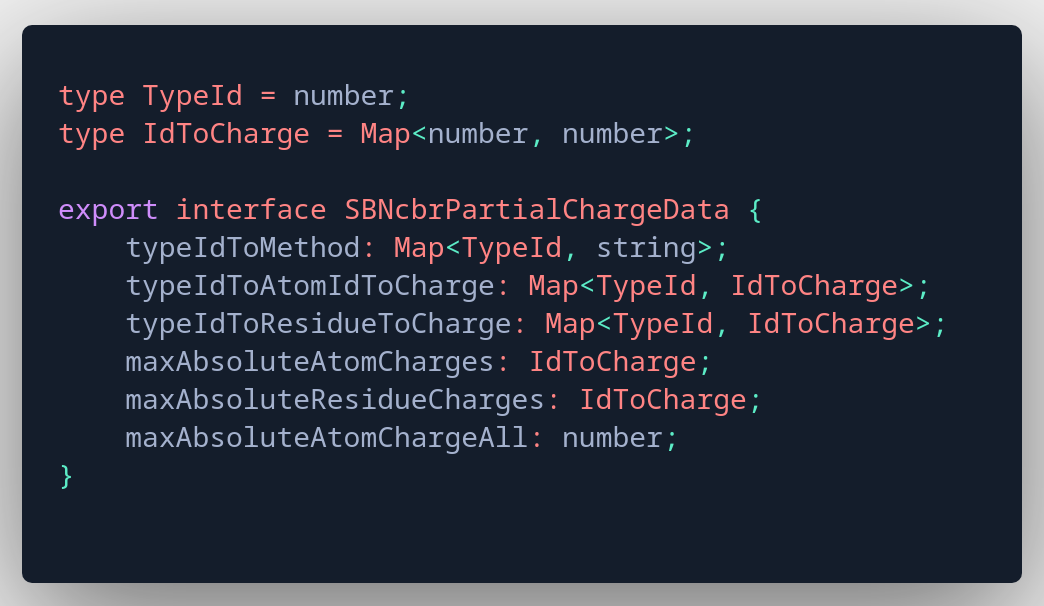
\includegraphics[width=10cm]{figures/charge_data_structure.png}
  \end{center}
  \caption{Structure of the custom model property used for storing the charges}
  \label{figure:charge_data_structure}
\end{figure}

This provider is responsible for supplying the partial atomic charges to the rest of the extension providers.
In order to retrieve the charges it is necessary to parse the mmCIF file.
This is fortunately already done by the Molstar library.
The library parses the mmCIF file and provides the parsed mmCIF file data in the form of a $\texttt{MmcifFormat}$ object.
This object is then used to retrieve the custom mmCIF categories described in Section \ref{section:custom_mmcif_categories}.

After retrieving the custom categories, the provider creates a custom model property for storing the charges. The interface depicted in Figure \ref{figure:charge_data_structure} describes the structure of the custom model property.

% \begin{itemize}
%   \item \texttt{typeIdToAtomIdToCharge} and \texttt{typeIdToResidueIdToCharge} - \\ map charges of a specific charge set (typeId) to the appropriate atoms or residues
%   \item \texttt{maxAbsoluteAtomCharges} and \texttt{maxAbsoluteResidueCharges} - \\ map the maximum absolute charge values for atoms or residues to a specific charge set (typeId)
%   \item \texttt{typeIdToMethod} - maps the charge set (typeId) to the method name used to calculate the charges 
% \end{itemize}

The atom charges are stored in the \texttt{typeIdToAtomIdToCharge} map. The map is indexed by the charge set (typeId) and the atom id. The atom id is a pointer to the atom\_site.id. item in the mmCIF file. The atom charges are retrieved from the mmCIF file by iterating over the atom\_site.id category and retrieving the charge values for each atom. The charge values are then stored in the \\ \texttt{typeIdToAtomIdToCharge} map.

The residue charges are calculated by summing the charges of the atoms that make up the residue. This is done by iterating over the atoms of the residue and summing their charges. The residue charge is then stored in the \texttt{typeIdToResidueIdToCharge} map. The maximum absolute charge of the residue is also calculated and stored in the \texttt{maxAbsoluteResidueCharges} map.

Lastly, the maximum absolute charge of both atoms and residues is calculated and stored in the \texttt{maxAbsoluteChargesAll} map and the method name used to calculate the charges of a given charge set is stored in the \texttt{typeIdToMethod} map.

\subsection{Partial charges color theme}
\label{subsection:partial_charges_color_theme}

This provider serves as the central component of the extension, with its primary function being to assign colors to atoms and residues based on their charges. It achieves this by using the ColorTheme API provided by Molstar. The ColorTheme API is a mechanism for assigning colors to structural elements of a molecule. These structural elements can be atoms, residues, bonds, and so on. The API is based on the concept of a ColorTheme object, which is a collection of color assignments for structural elements. The ColorTheme object is then used by the Molstar library to color the structural elements of the molecule.

For the purposes of this extension, it was necessary to color two structural elements - atoms and residues. For both of these structural elements the charges were retrieved from the provider described in the previous section \ref{subsection:charges_provider}, which provided charges for atoms and residues.

To establish the color for a given charge, two color interpolations are employed: one for negative charges and another for positive charges. Atoms with positive charges receive a color from a white-to-blue color interpolation, while atoms with negative charges are assigned a color from a white-to-red color interpolation. These color interpolations are highlighted in Figure \ref{todo}. 

\subsection{Labels}
\label{subsection:labels}

Having colored the structural elements, it was also necessary to create a label provider, which would assign labels that describe the charge of the structural element. In order to determine which element is highlighted, Molstar uses the object Loci. A Loci object is utilized for general selections and highlights. Consequently, it is essential to first extract the location from the Loci object in order to obtain the atom ID. The charge is acquired from the property provider, and the label is an HTML string that conveys the charge of the atom or residue. An example of the label can be seen in in the right-hand corner in figure \ref{}.

\section{Molstar integration}

After creating the extension, it was integrated into the Molstar library. The extension is integrated in a way that allows the user to simply upload a mmCIF file together with the custom charge categories in the Molstar viewer. The color theme is set automatically to the partial atomic charge color theme. By integrating it into the Molstar library the extension was made freely available to anyone to use

\section{Future work}

The extension can be improved in many areas - mainly in the UI. It can be optimized by storing the atom and residue charge maps statically. The extension unnecessarily recalculates the maps when switching to another charge set. Another area that could use some work is the UI. When a user wants to switch to another charge set, they need to use the State Tree UI. If the user has only one structure loaded, this is fine. However, once you have more than one structure and want to change the charge set for each one of them, then it becomes very tedious. A better approach is to create a custom UI element in the right sidebar which would serve as a shortcut to set a charge set globally or for each structure individually. Another custom UI control could be used for setting a global max absolute charge - this is also done manually for each structure.

\chapter{Molstar viewer plugin}

TODO: maybe make this a section in chapter about ACC2 \\

In addition to creating the partial atomic charges extension for Molstar, it was necessary to create a custom Molstar viewer instance to facilitate custom functionality not present in the official Molstar viewer instance deployed at molstar.org/viewer. This chapter focuses on describing the implementation and functionality of the custom Molstar viewer instance for the web applications discussed in chapters 5 and 6.

\section{Requirements}

The viewer needs extended functionality

\chapter{Atomic Charge Calculator II}
\label{chapter:atomic_charge_calculator_ii}

Atomic Charge Calculator II (ACC2) is a web application for calculating and visualizing partial atomic charges. ACC2 uses the Litemol viewer for visualizing the structures and their partial atomic charges. The viewer is sufficient in visualizing a single charge set, however, it was desired to expand this capability to support multiple charge sets. This is why it was desirable to update the viewer with its modern counterpart Molstar, which has this capabilty provided through the partial atomic charges extension described in chapter \ref{}.

This chapter discusses the necessary changes made to the ACC2 web application in order to update the viewer from the Litemol viewer to the Molstar viewer. Firstly, we discuss the extensions made to the ChargeFW2 output, then we will look at the Flask backend changes for supporting multiple charges, and lastly we will mention a couple of frontend changes that were made to support generating multiple charge set calculations.

\section{ChargeFW2 extension}
\label{section:chargefw2_extension}

As mentioned in subsection \ref{}, ChargeFW2 is a C++ application for calculating partial atomic charges.
To accommodate the specified output file format discussed in section, ChargeFW2 required an extension that would output a single mmCIF file containing both the molecular structure and charges. The charges were appended to the end of the file.jop

\section{Multicharge support}
\label{section:multicharge_support}

\subsection{Backend}

\subsection{Frontend}

\section{Molstar viewer integration}

\chapter{AlphaCharges}

\section{Viewer extension}

\section{Molstar viewer integration}

\chapter*{Conclusion}
\markright{\textsc{Conclusion}}
\addcontentsline{toc}{chapter}{Conclusion}

Things were created and some things even work.

\end{document}
